\documentclass[a4paper,11pt,notitlepage]{article}
\usepackage[margin=2cm]{geometry}
\usepackage{fancyhdr}
\usepackage{amsmath}
\usepackage{textcomp}
\usepackage{enumitem}
\usepackage{graphicx}
\usepackage{tabularx}
\usepackage{subcaption}
\usepackage{wrapfig}
\usepackage[section]{placeins}

\usepackage[nodayofweek]{datetime}
\longdate

\usepackage{fancyhdr}
\fancyhf{}
\lhead{\fancyplain{}{M.Sc.\ Individual Background Report}}
\rhead{\fancyplain{}{\today}}
\cfoot{\fancyplain{}{\thepage}}


\title{Cyclist Collision Detection in Urban Environments \\\Large{--- Background Report ---}}
\author{Peter Hedley\\
       ph817@doc.ic.ac.uk\\ \\
       \small{Supervisor: Dr.\ Stefan Leutenegger}\\
       \small{Course: CO541, Imperial College London}
}


\begin{document}
\maketitle

\begin{abstract}
This report investigates the use of existing state of the art image detection, segmentation and SLAM algorithms for use by cyclists in urban environments. The challenges facing cyclists in a daily commute include monitoring pedestrian movement, vehicle movement and obeying the rules of the road. The aim of the project is to provide a detection system to enable safer cycling on dangerous city-roads.

\end{abstract}
\clearpage

\tableofcontents

\clearpage
%%%%%%%%% PART 1 - Status: done %%%%%%%%%%
\section{Introduction}
There were c. 18,500 cycling accidents and 3,500 deaths on British roads in 2016 \cite{DFT_fig}. Of these accidents 80\% occur during the day and driver/rider error accounts for 71\% of the total collisions \cite{DFT_fig2}. The most common place for a cycling incident is at a road junction with 75\% of collisions occurring there \cite{DFT_fig3}. With cycling becoming a more accepted form of transport, the need to protect and modify bikes with a comprehensive safety system is important.
\newline\newline
This report will examine state of the art technologies that are used for autonomous vehicles to investigate their applicability to a cycling environment. The three main topics involve image detection/segmentation, SLAM algorithms and collision/path prediction. 

\newpage
\section{Background, Computer Vision}\label{comp_vis_back}
\subsection{Deep Learning Preliminaries}
Computer vision and its applications has been revolutionised recently by Deep Learning frameworks. These have led to super-human accuracy in image recognition, for example Inception v3 \cite{Szegedy_2016_CVPR}, release in 2016, reached a 3.46\% error rate on the ImageNet \cite{ILSVRC15} dataset. This is known of as an image classification task; the photo contains one object in the dataset and that object generally occupies the majority of the frame. Similar networks are used with additional features for image detection and segmentation which are integral to detecting moving objects such as pedestrians and vehicles in an urban environment.
\newline\newline
The current state-of-the-art methods in computer vision use a form of neural network. These networks are characterised by a series of non-linear nodes that are organised in layers. At each layer the network learns progressively abstract and higher-level features of the image to be detected until the final (usually dense layer) at the end which determines the predicted class. Therefore the 'depth' of a neural network often refers to the number of layers and hence the inherent complexity of features that a network can learn. This is, however, only a basic representation of the problem and some clever and shallower architectures are able to outperform deeper networks. It is important to note that the depth and width, more specifically the number of parameters in the model generally reduces speed of prediction and increases the memory required to store/load the model into RAM. This is of little consequence in most applications, however for the limited computational power able to be carried on a bicycle it will be of concern in this report.

\subsection{Convolutional Networks} \label{Cnn_section}
A CNN generally contains convolutional, pooling, fully connected and normalisation layers. This form of network became particularly popular in computer vision after Geoffrey Hinton's 2012 paper \cite{GH_CNN}, with an ImageNet classification error of c.16\%, significantly lower than the state-of-the-art at the time 26\%. Convolutional networks use the assumption that each input is an image and therefore certain properties can be encoded into the architecture of the network. This allows a significant reduction in the number of network parameters to tune.
\newline \newline
A regular neural network, as mentioned earlier, contains a number of fully connected layers i.e. each neuron in a layer is connected to every neuron in the previous and next layers respectively. However convolutional neural networks are arranged in three dimensions: width, height, depth (Figure \ref{CNNvsNN}). In this architecture the neurons in a layer are only connected to some of the layer before unlike in the fully connected case, this significantly reduces the number of parameters \cite{StanfordCS231_1}.

\noindent \begin{figure}[h!]
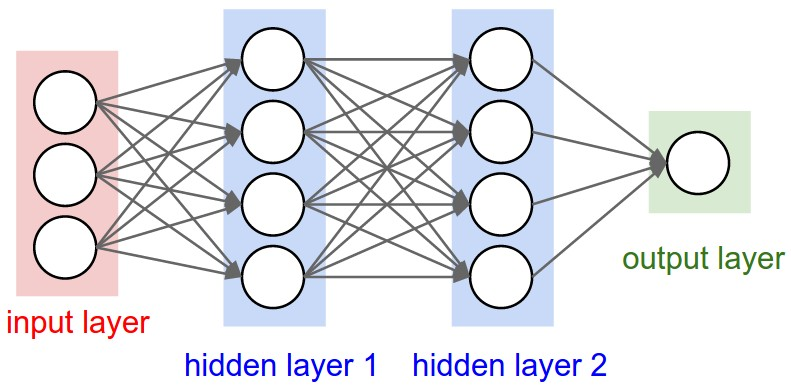
\includegraphics[width = 0.5\hsize]{./figures/neural_net2.jpeg}
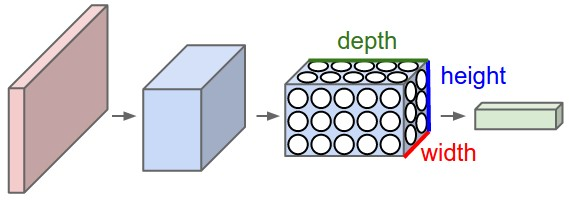
\includegraphics[width = 0.5\hsize]{./figures/cnn.jpeg}
\caption{Regular Neural Network (Left) \cite{StanfordCS231_1} , CNN (right) \cite{StanfordCS231_1}.}
\label{CNNvsNN}
\end{figure}

\subsubsection{Convolutional Layers}
A convolutional layer learns a set of filters, each filter is compact in size, say ($7 \times 7 \times 3$). This filter slides (convolves) over the image, then a dot product is taken between the filter values and the inputs to that filter (Figure \ref{CNN_filter}. The filter slides across with a respective stride, which is a hyperparameter, a stride of one equates to moving one pixel across at a time. A convolutional layer is therefore able to pick up features such as a corner, or higher level features such as the texture of fur. This process creates a 2D activation map containing the response of the filter at each position on the input volume. A number of filters are passed over and a number of activation maps created, relating to the depth which is a tune-able hyperparameter.

\noindent \begin{figure}[h!]
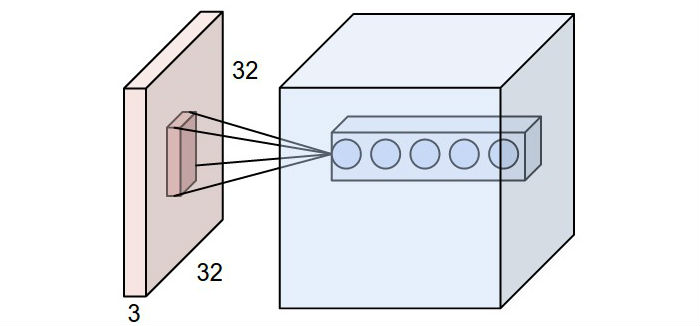
\includegraphics[width = 0.5\hsize]{./figures/conv_filter.jpg}
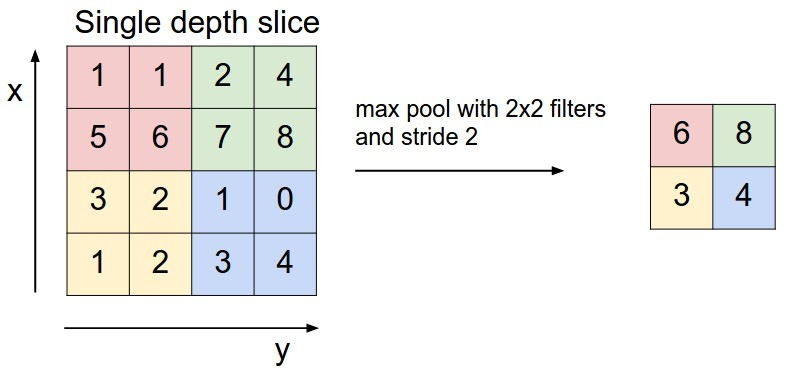
\includegraphics[width = 0.5\hsize]{./figures/maxpool.jpeg}
\caption{CNN Filter (left) \cite{StanfordCS231_conv_filter}, Max Pooling \cite{StanfordCS231_max_pool}}
\label{CNN_filter}
\end{figure}

\subsubsection{Pooling Layers}
Pooling layers are used to reduce the number of parameters in a network. This is a much debated topic, Geoffrey Hinton's \cite{DBLP:journals/corr/abs-1710-09829} dicusses the problems of convolutional networks in his 2017 paper and especially focuses on the disadvantages of pooling layers. It is however a current, although fading, method of parameter reduction. For the purposes of optimising network architecture for smaller hardware such as is portable on a bike this is still a recognised and useful method.
\newline \newline
A pooling layer such as that depicted in (Figure \ref{CNN_filter}) passes a kernel over the input (much like in a convolutional layer) and at each spacial location it calculates a metric. For example, max pooling takes the largest value contained within the kernel grid at each consecutive spacial location.

\subsection{Image Detection} \label{Image_det}
Image detection is an area of research that uses the CNN networks described in Section \ref{Cnn_section}. This is, however, a more difficult task as there can be multiple objects/classes of interest within one image. A naive approach to this problem would be to slide a window across an image and classify at each location. When the network classifies, say a cat at a particular window location it is likely that a cat is located in that area.
\newline \newline
Although the aforementioned approach is valid it would be very slow, not only would it be needed to slide the window over the whole image, the size of the window would also need to be varied. The network cannot know the area of the photo that the object occupies and therefore what size to make the window. There are a number of differing approaches to this problem R-CNN \cite{DBLP:journals/corr/GirshickDDM13} and other later iterations vs YOLO (you only look once) \cite{DBLP:journals/corr/RedmonDGF15}. The R-CNN approach is very similar to the vanilla, naive solution, discussed above (commonly known as exhaustive search) and is used by later techniques for instance segmentation.


\subsubsection{R-CNN} \label{rcnn}
R-CNN, proposed by Ross Girshick et al. \cite{DBLP:journals/corr/GirshickDDM13} in 2014, incorporates a region proposal method. This process produces 2000 proposals which are then classified by a large CNN classifies each region using class-specific linear SVMs. This process equates to a 53.7\% mean average precision (mAP) compared to 35.1\% by the current state-of-the-art at the time. In addition to this performance gain the system doesn't rely on far more complicated ensemble methods.
\newline \newline
The region proposal method used is called selective search \cite{Uijlings2013} , this uses a fast segmentation algorithm by Felzenszwalb \cite{Felzenszwalb2004} followed by a greedy algorithm to iteratively group regions together using a similarity metrics. The four metrics proposed in the paper are $s_{colour}$, $s_{texture}$, $s_{size}$, $s_{fill}$  the aim is to use a number of metrics to pick up the differences between regions when growing and also limit one region's growth at the expense of others (hence the size metric).

\noindent \begin{figure}[h!]
\label{Selective_search}
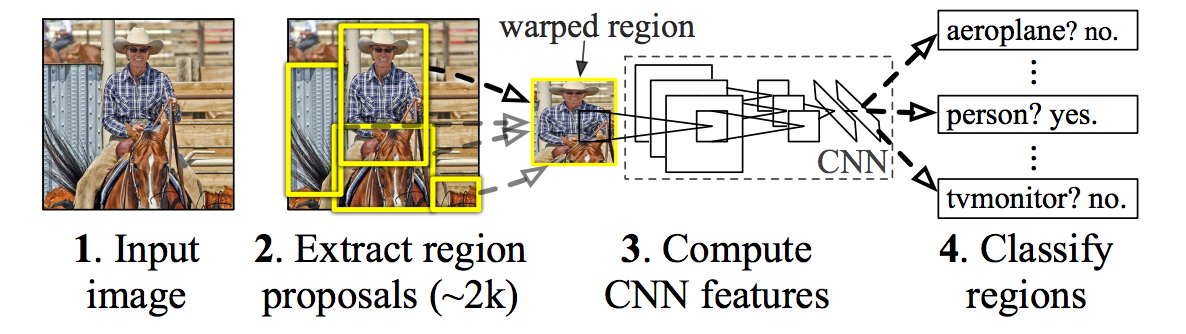
\includegraphics[width = 1.0\hsize]{./figures/region_prop.png}
\caption{R-CNN Region Proposal \& Architecture \cite{DBLP:journals/corr/GirshickDDM13}}
\end{figure}

The result of the region proposal (Figure \ref{Selective_search}) are a series of windows that are likely to contain an object. These are then simply warped to $227 \times 227$ pixels to fit the input dimensions CNN network that contains five convolutional layers and two fully connected layers. The output of the CNN is then fed as a 4096 dimensional feature vector to a set of trained SVMs, one for each class, that are used to score the likelihood for that class. This approach is slow at 13s/image on a GPU and 53s/image on a CPU, the separation of a CNN and SVM is peculiar and adds to this timescale. A later iteration of this method Fast-RCNN is discussed in Section \ref{Fast_RCNN}.

\subsubsection{Fast-RCNN} \label{Fast_RCNN}

R-CNN performs a CNN forward pass for each region proposal and does not share computation \cite{DBLP:journals/corr/Girshick15}. Spacial pyramid pooling networks (SPPnet) \cite{DBLP:journals/corr/HeZR014} are designed to mitigate this problem by creating a feature map (which is always the same shape) from an input image and then classifies each object proposal from a vector extracted from the shared feature map. This paper still uses a multiple-stage classification pipeline but is a marked improvement on R-CNN with regards to speed. 

Fast-RCNN uses the SPPnet concept but also incorporates a single-stage pipeline. The process inputs an image and multiple RoIs into a fully convolutional network (Figure \ref{Fast_RNN}). Each RoI is then pooled into a fixed-size feature map as in SPPnet and then mapped to a feature vector by fully connected layers. As can be seen in Figure \ref{Fast_RNN} the network then branches into 2 separate outputs, one 4-point regression output of the bounding box location and a K-size classification output, where K is the number of object classes. The model therefore must contain a multi-task loss function that accounts for both bounding box and softmax loss (Equation \ref{multi-task_loss}).

\begin{equation}
\label{multi-task_loss}
L(p,u,t^{u},v) = L_{cls}(p,u) + \lambda[u \geq 1]L_{loc}(t^{u},v)
\end{equation}
in which $L_{cls}(p,u) = -log(p_{u})$ is the log-loss for true class $u$, and $L_{loc}$ is the bounding box regression loss defined as:

\begin{equation}
\label{bbox_loss}
L_{loc} = \sum_{i\in \{x,y,w,h\}}smooth_{L_{1}}(t^{u}_{i}-v_{i}),
\end{equation}
in which

%TODO
\begin{equation}
\label{multi-task_s}
smooth_{L_{1}} = 
\begin{cases}
0.5x^{2} \textnormal{if} x < 1 \\
|x| - 0.5  \textnormal{otherwise} \\
\end{cases}
\end{equation}
is a $L_{1}$ loss. This architecture allows for fast training with the forward pass of the network and therefore processes images 146$\times$ faster than R-CNN. 

%TODO
\noindent \begin{figure}[h!]
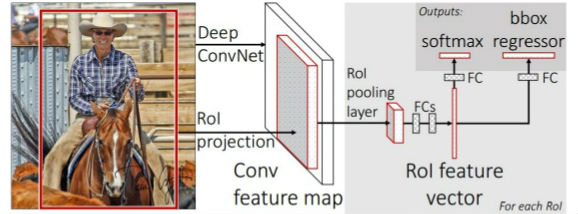
\includegraphics[width = 1.0\hsize]{./figures/fast-rcnn2.jpg}
\caption{Fast R-CNN Architecture \cite{DBLP:journals/corr/Girshick15}}
\label{Fast_RNN}
\end{figure}

Figure \ref{Fast_RCNN} depicts the pipeline architecture, this incorporates an RoI pooling layer which maps the convolutional feature map from an RoI (created by selective search) to a fixed extent feature map of a set $H \times W$, where $H$ and $W$ are layer hyperparameters. Each RoI is a rectangular window defined by a tuple of four elements ($r,c,h,w$), where ($r,c$) specify the top left corner and ($h,w$) the width. RoI max pooling then divides the RoI window into a grid and then max-pools each grid into the corresponding output cell. The size of the grid is proportionate to the RoI and so the output shape is constant regardless of RoI input size. 

\subsubsection{Faster R-CNN} \label{Faster_rcnn}
Although the previous method \cite{DBLP:journals/corr/Girshick15} removed the need for a multi-stage classification pipeline (CNN and SVM), it still relies on the selective search \cite{Uijlings2013} method for region proposal. This part is now the computational bottleneck that slows down the process. Faster R-CNN proposed by Ren et al. \cite{DBLP:journals/corr/RenHG015} seeks to alleviate this issue by combining region proposal into the CNN. The paper suggests the use of a region proposal network (RPN) to produce the RoIs used later in the network. 

%TODO sort out grphic keep only (c)
\noindent \begin{figure}[h!]
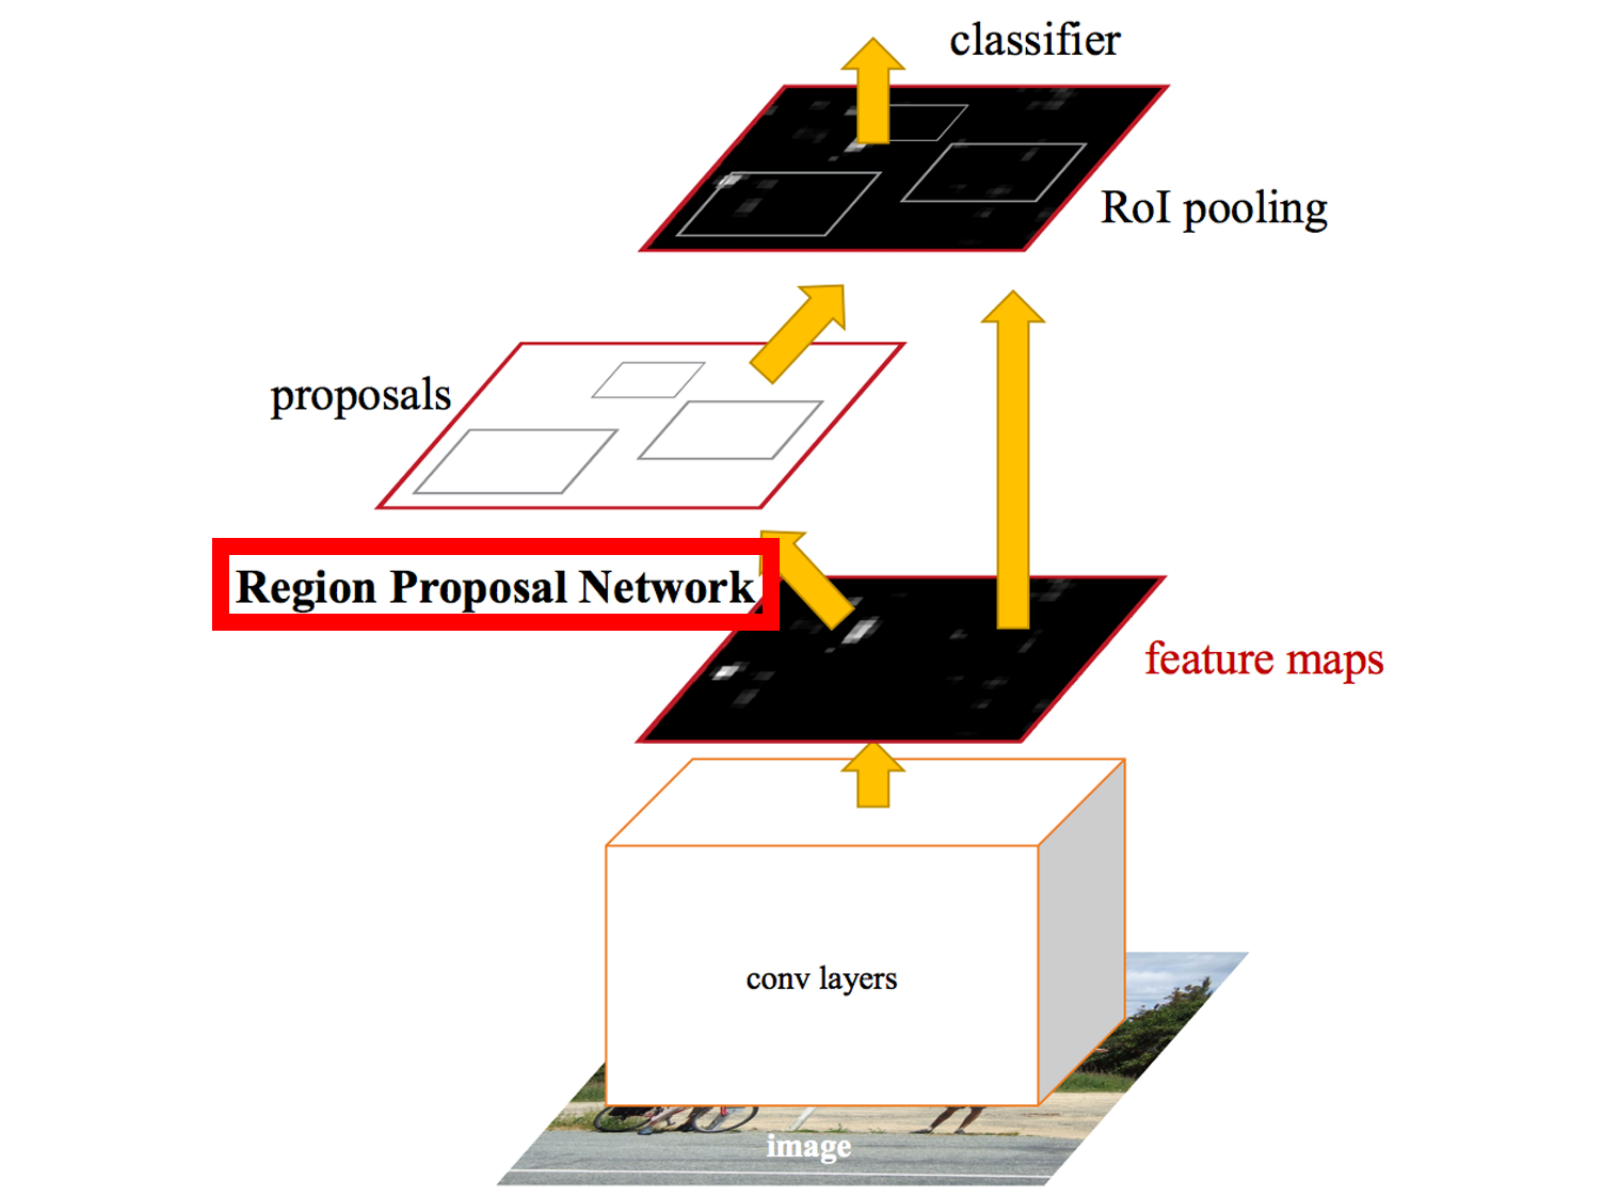
\includegraphics[width = 0.5\hsize]{./figures/faster.png}
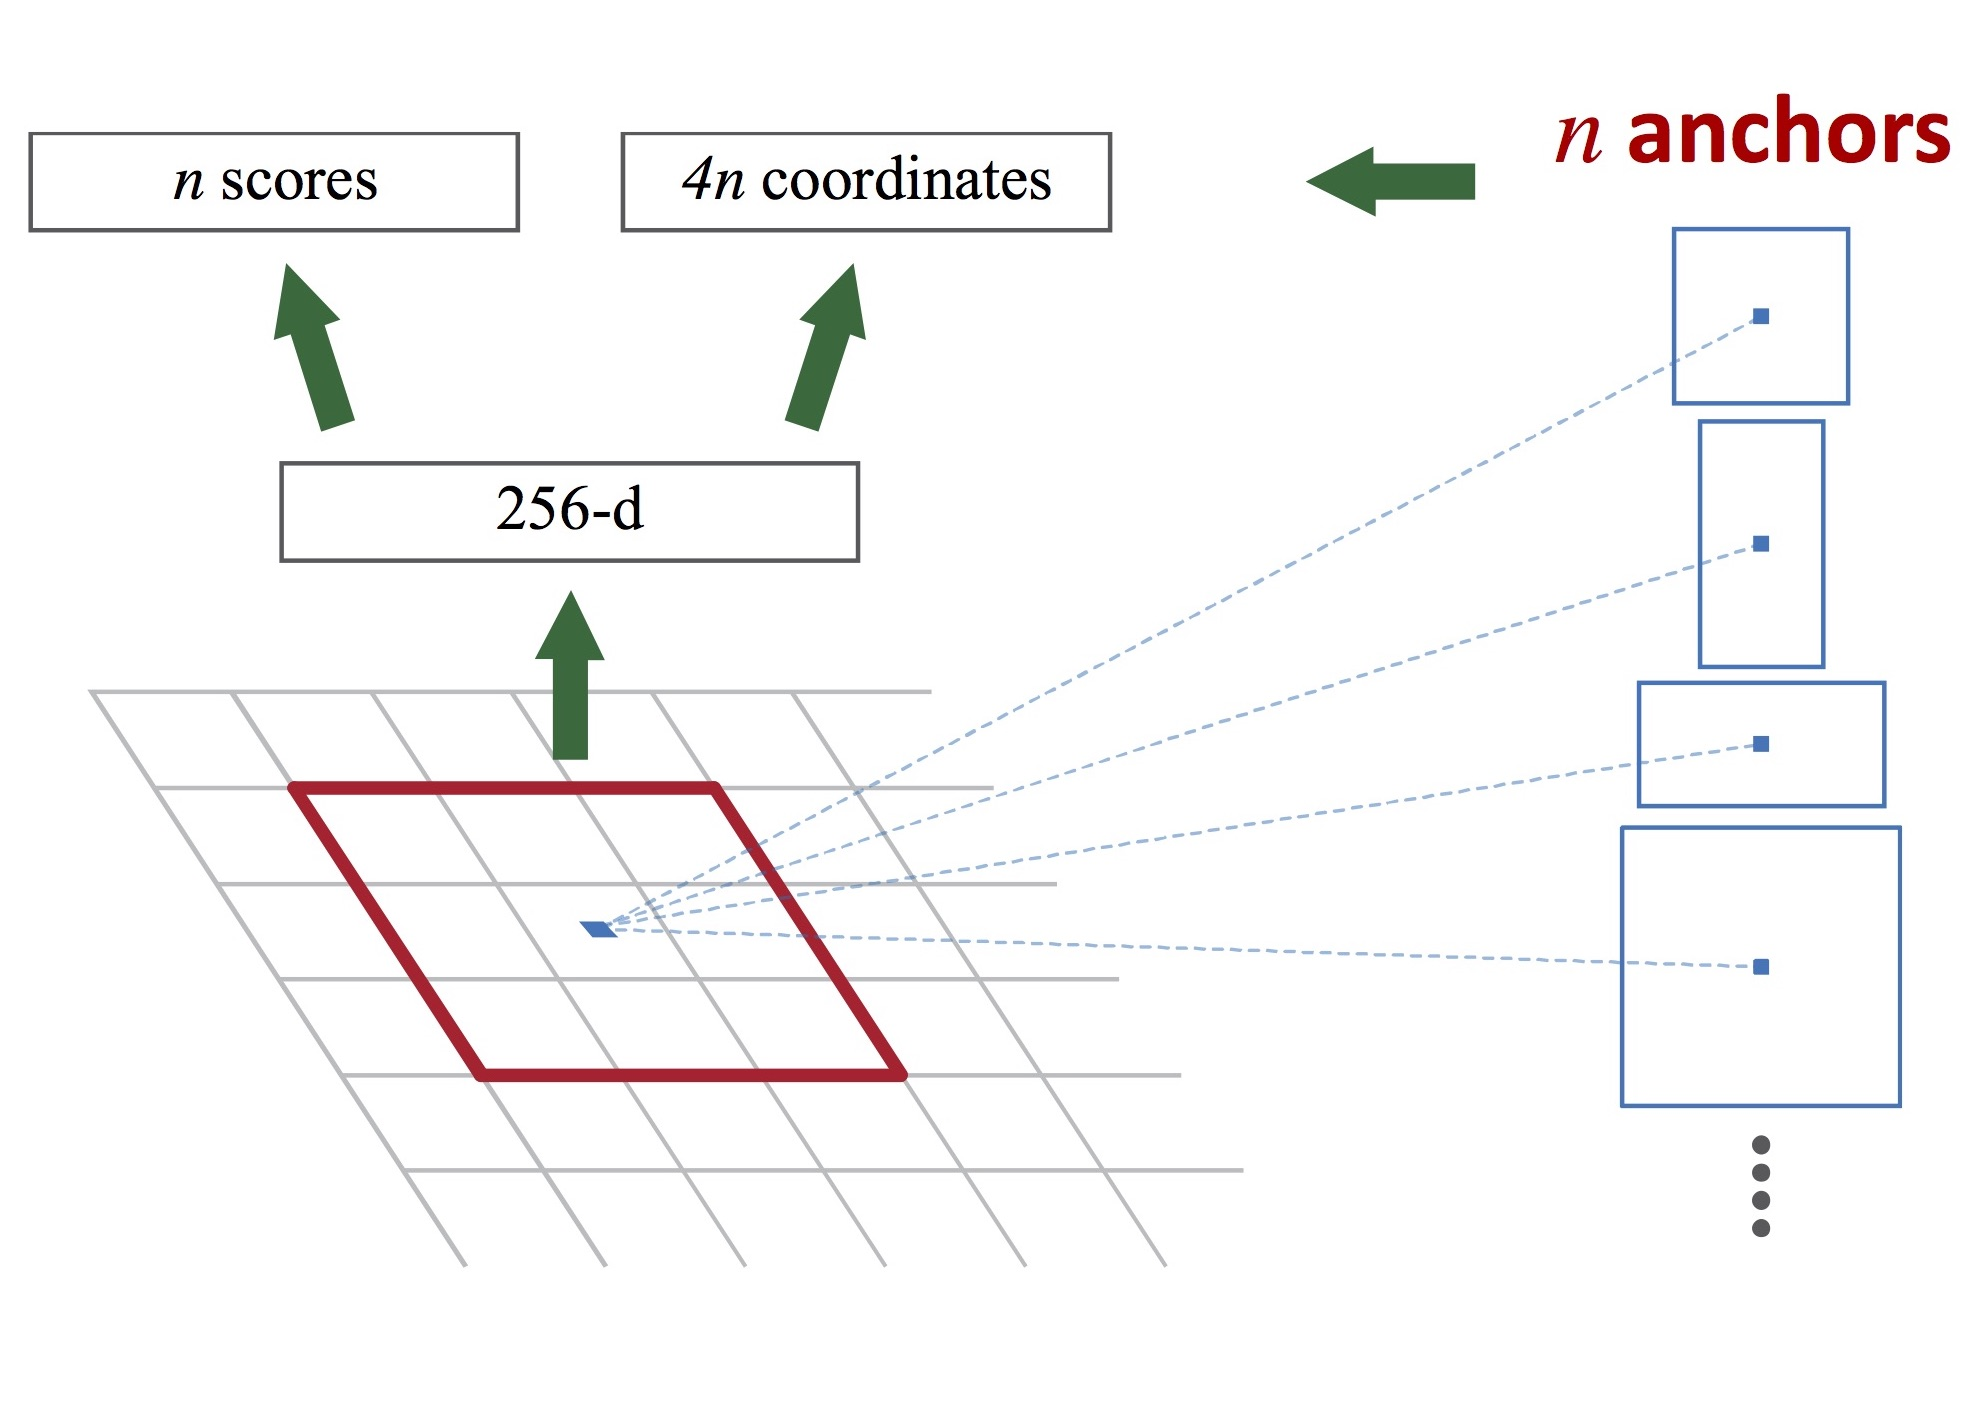
\includegraphics[width = 0.5\hsize]{./figures/rpn_faster.jpg}
\caption{Fast R-CNN Architecture \cite{DBLP:journals/corr/Girshick15}}
\label{Faster_rnn_fig}
\end{figure}

The region proposal network (RPN) outputs a set of rectangular object proposals, each of these proposals has an objectiveness score i.e. how likely the network thinks the proposal contains an object. This part of the network comes after a number of convolutional layers (in this paper 5 or 13 such layers). The region proposals are then created off the feature map from these layers by sliding a smaller network of size $n \times n$ over the convolutional feature map (Figure \ref{Faster_rnn_fig}. At each sliding window location a number of region proposals are predicted simultaneously. These consist of 3 aspect ratios and 3 scales, therefore 9 total region predictions or anchors at each location. The network is then followed by two sibling $1 \times 1$ convolutional layers, one for $reg$ (region proposal) and one for $cls$ (probability of object or not). The $reg$ layer outputs 4$k$ results, which represent the encoding coordinates of the $k$ boxes and the $cls$ later scores the probability that there is an object or no object in each proposal, therefore $2k$ outputs. This results in a convolutional layer output of depth 9.

The loss for the network is calculated from two metrics, the output of the $reg$ layer is a binary i.e. positive example or not. A positive example is defined by how much the box overlaps with the ground truth box of the object and so an IoU (Intersection-over-union) overlap > 0.7 is considered a positive example and an IoU < 0.3 is considered a negative label. For the first positive case if no positive examples are found the boxes with highest IoU  are labelled positive. With this it follows that:

\begin{equation}
\label{multi-task_loss}
L(\{p_{i}\},\{t_{i}\}) = \frac{1}{N_{cls}} \sum_{i} L_{cls}(p{i},p_{i}^{*}) + \lambda \frac{1}{N_{reg}} \sum_{i}p_{i}^{*} L_{reg}(t_{i},t_{i}^{*})
\end{equation}

Where $i$ is the anchor index, $p_{i}$ is the predicted probability of anchor $i$ containing an object. The ground truth label $p_{i}$ is denoted as a 1 for a positive anchor and 0 for a negative therefore $L_{reg}$ is only activated for a positive example, $t_{i}$ and $t_{i}^{*}$ represent the 4 coordinates of the bounding boxes, and $L_{cls}$ is the classification loss. The two terms are normalised ($N_{cls}$ and $N_{reg}$) and balanced by a weighting parameter $\lambda$. The final term to discuss, the bounding box regression is calculated, simply, as follows:

\begin{equation}
\begin{aligned}
\label{multi-task_loss}
t_{x} = (x-x_{a})/w_{a}, \quad t_{y} = (y-y_{a})/h_{a},\\
t_{w} = log(w/w_{a}), \quad t_{h} = log(h/h_{a}), \\
t_{x}^{*} = (x^{*}-x_{a})/w_{a},\quad t_{y}^{*} = (y^{*} - y_{a})/h_{a} \\
t_{w}^{*} = log(w^{*}/w_{a}), \quad t_{h}^{*} = log(h^{*}/h_{a})
\end{aligned}
\end{equation}

where $x$, $y$, $w$, and $h$ are the box centre coordinates plus width and height. Predicted box, anchored box are denoted by $x$, $x_{a}$, $x^{*}$ (likewise for $y$, $w$, $h$).

Finally after the regions have been proposed c.6000 per image, some regions overlap with others, and so, to reduce redundancy non-maximum supression is used on their cls score with an IoU threshold of 0.7 to leave around 2000 proposals per image. Non-maximum supression is a technique that sets all neighbouring areas to zero around a local maximum and hence only keeps the maximum value and suppresses the others.
 
\subsection{Image Segmentation}\label{image_seg}
Unlike the image detection problem described in Section \ref{Image_det}, this task aims to segment an image on a pixel-by-pixel basis into respective classes (Figure \ref{cityscapes_data}). A conventional classification network takes an image and outputs a prediction of which class the image is i.e. a vector of probabilities or a `score'. This process uses fully-connected layers to produce the final output vector which throws away important spacial information used in a segmentation task. Therefore Long et al. \cite{DBLP:journals/corr/LongSD14} propose converting these final layers to convolutional layers, maintaining the spacial information and creating a heatmap output (Figure \ref{cityscapes_data}).

\noindent \begin{figure}[h!]
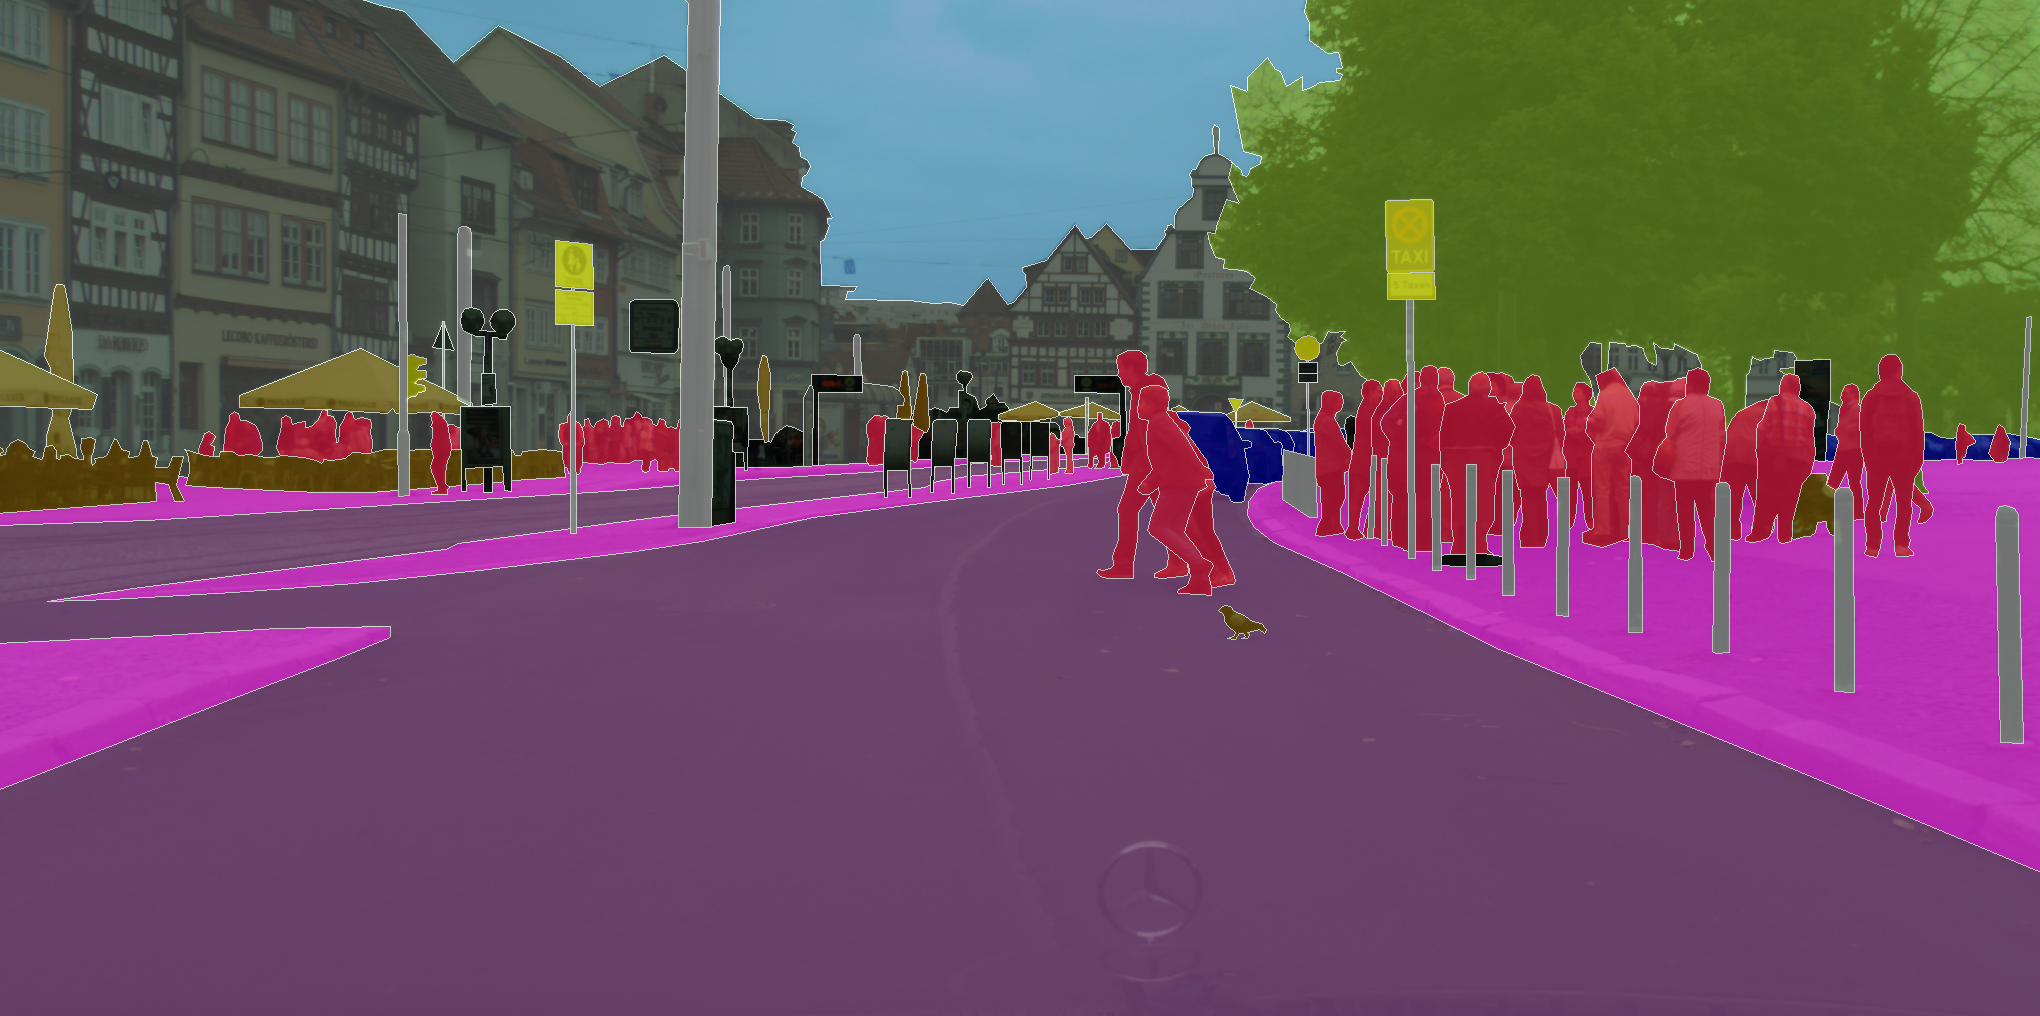
\includegraphics[width = 0.5\hsize]{./figures/image_seg1.png}
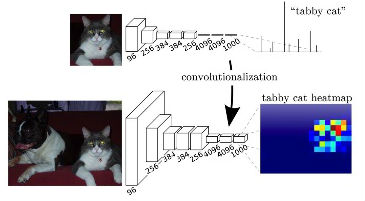
\includegraphics[width = 0.5\hsize]{./figures/sem_im_seg1.jpg}
\caption{Image Segmentation \cite{DBLP:journals/corr/CordtsORREBFRS16}, Convolutional Heat Map \cite{DBLP:journals/corr/LongSD14}}
\label{cityscapes_data}
\end{figure}

The heatmaps produces from the network then need to be upsampled from their respective dimensions to that of the output image. This process is essentially a reverse or deconvolution. Upsampling, therefore, with factor f is convolution with a fractional input stride of 1/f. Essentially each filter is placed on the output image and then multiplied by the input pixel. Hence the image increases in size depending on stride and kernel size as one pixel value is interpolated over a grid. The final problem therefore is how to choose the filter values, this can be done in a number of ways but the main accepted approach is to simply learn them as part of the tuning process.
\newline \newline
An important concept is that of patchwise training which feeds the network a number of patches from an input image (small patches surrounding objects of interest) instead of an entire input image. This both helps to balance the classes, ensures the input has enough variance, and is a correct representation of the input set. However, this paper argues that this can be done from a fully convolutional training regime with incorporating a DropConnect-like mask \cite{Wan:2013:RNN:3042817.3043055} between the output and the loss. A DropConnect mask is similar to the proposed regularisation technique of Dropout \cite{JMLR:v15:srivastava14a} except that it randomly sets the network weights to 0 rather than the activation functions. This, on the output layer (connected to the network loss) is found to have the same effect as patch-wise sampling in Long et al.'s paper.
\newline \newline
Although conventional, proven classification architectures performed to state-of-the-art when modified for segmentation 56.0 mean IU it was found that a novel and specific architecture performed best 62.7 mean IU. Mean pixel intersection over union (Mean IU) is a standard performance metric where mean is taken over all classes, including the background. The paper describes a network architecture that uses skips \cite{Bishop:2006:PRM:1162264}. Skips allow predictions from lower-level coarser layers to interact with finer, latter layer predictions. This lets the model make local predictions (finer) within the context of the global structure (coarser). This addition made for a marked increase in performance by simply up-sampling earlier layers and summing with latter layer outputs for a final image prediction.

\subsection{Instance Segmentation}
Instance segmentation is a problem that combines research in Sections \ref{Image_det} \& \ref{image_seg}, it aims to not only perform pixel-wise segmentation of classes but also determine instances of objects within and image. As discussed in Section \ref{mask_rcnn} there is a simple method of combining these networks into one simple classification pipeline.
\subsubsection{Mask R-CNN} \label{mask_rcnn}
Mask R-CNN was proposed by Facebook AI Research (FAIR) namely Kaiming He et al. in March 2017. It uses the Faster R-CNN network described in Section \ref{Faster_rcnn} which builds from advances in Sections \ref{rcnn}  \& \ref{Fast_RCNN}. The method works by simply adding a branch from the existing network for predicting segmentation masks as in Section \ref{image_seg} (Figure \ref{Mask_rcnn_arch}). The branch is a small FCN that is applied to each ROI for segmentation. There are a number of slight modifications to each approach to produce the final Mask R-CNN that are documented below.


\noindent \begin{figure}[h!]
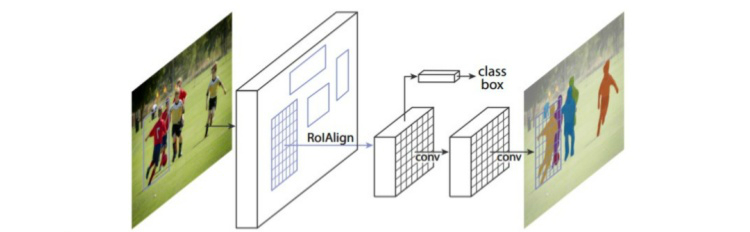
\includegraphics[width = 1.0\hsize]{./figures/mask_arch.jpg}
\caption{Mask R-CNN \cite{DBLP:journals/corr/HeGDG17}}
\label{Mask_rcnn_arch}
\end{figure}
%TODO nice binary mask per class photo
RoIs are produced from the RPN as in Faster R-CNN \cite{DBLP:journals/corr/RenHG015} then an $m \times m$ mask is predicted from each RoI without the use of a fully-connected (fc) layer and therefore keeps spacial information as in Section \ref{image_seg}. It was found during experimentation that it is preferable to decouple the class classification and the mask production of the network. This stops multiple classes disrupting each-other during mask production, hence a mask is produced for each class. The class of each respective mask is then determined from the class output branch and that binary mask is selected. 
\newline \newline
The loss function for the network must now incorporate the three different branches; mask, class prediction, bounding-box prediction (Equation \ref{maskrcnnloss}). 

\begin{equation}
\label{maskrcnnloss}
L = L_{cls} + L_{box} + L_{mask}
\end{equation}

Where $L_{cls}$ \& $L_{box}$ are identical to Section \ref{Fast_RCNN}. The mask branch loss is determined by a per-pixel sigmoid between the ground-truth class ($k$) and the corresponding $k$th binary mask (excluding other classes) and is calculated with an average binary cross-entropy loss.
\newline \newline
RoI pool as discussed in Section \ref{Fast_RCNN} is modified in this approach. Instead of subdividing an RoI into discrete regions e.g. a grid of $4 \times 5$ cells. An RoI does not always divide equally into these grid cells and so rounding of grid sizes is needed, this quantisation of sub-windows can cause misalignments of the RoI and extracted features. The new RoIAlign layer introduced in this paper mitigates this problem by not rounding grid-cells. Mask R-CNN uses bi-linear interpolation (linear interpolation with 2d) to compute the exact values of input features at four regularly samples locations in each RoI window.

\section{Background, SLAM}
In order to detect collisions between the bike and obstacles the software must have an understanding of the global environment. The detection described in Section \ref{comp_vis_back} allows mapping, and tracking of dynamic objects in the frame, but distance, path prediction and eventually collision prediction rely strongly on an accurate understanding of 2.5-3D space.

\subsection{Sensors}
The sensors used in this project are an RGBD camera and an IMU. These are both available in the Intel Realsense Camera (ZR300, Figure \ref{realsense_camera}). This camera has a USB cable that both provides the power and sends camera information. An extension cable allows for a laptop to be attached to the camera, from a backpack whilst cycling. Potential problems with this setup are due to the potential juddering of the bike during operation. This could cause tricky footage to analyse and can cause data loss when the hard-drive is writing to disk. The later issue can been easily solved by writing to an SSD while cycling.

\noindent \begin{figure}[h!]

\includegraphics[width = 1.0\hsize]{./figures/intel_realsense.jpg}
\caption{Intel Realsense Camera (ZR300)}
\label{realsense_camera}
\end{figure}

\subsection{World and Camera Frame}



In order to fully understand the bike's location, the environment can be considered from two frame's of reference, the world and camera frame. 
\newline


\noindent \begin{figure}[h!]
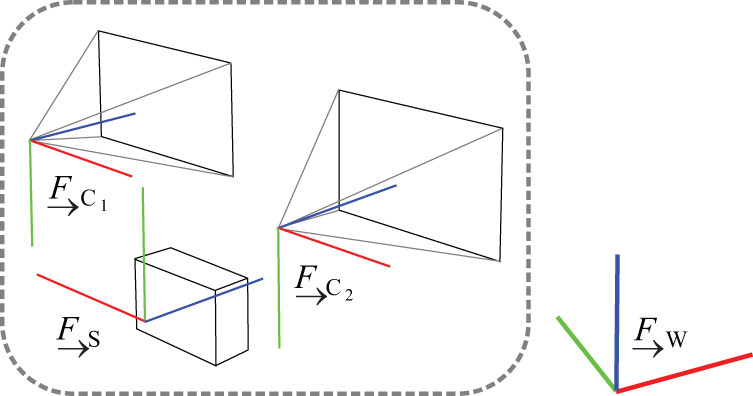
\includegraphics[width = 0.5\hsize]{figures/world_to_cam.jpg}
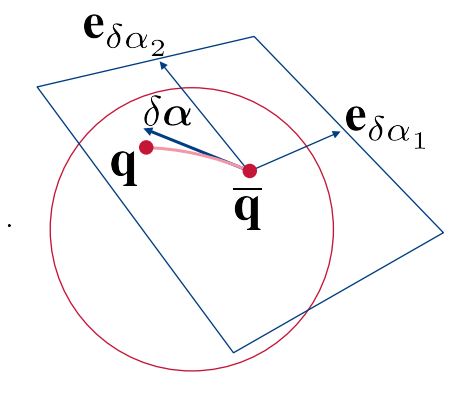
\includegraphics[width = 0.35\hsize]{figures/quaternions.png}
\caption{World vs Camera Frame \cite{Okvis_1}}
\label{quat_wcs}
\end{figure}


\iffalse
\begin{wrapfigure}{r}{0.5\textwidth}
  \begin{center}
    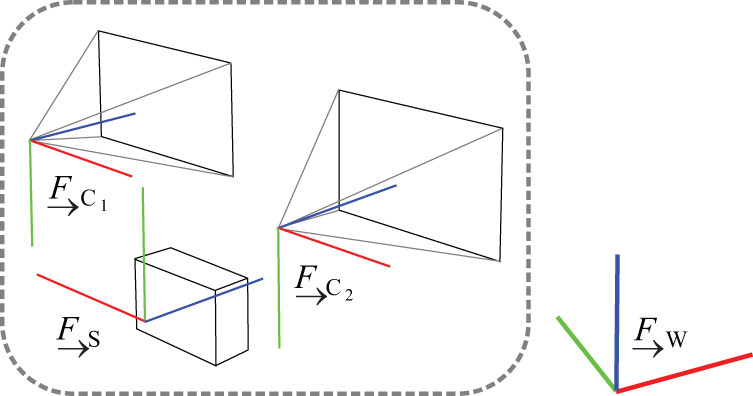
\includegraphics[width=0.48\textwidth]{figures/world_to_cam.jpg}
  \end{center}
  \caption{World vs Camera Frame \cite{Okvis_1}}
\end{wrapfigure}
\fi
To convert between world (${\xrightarrow{F}}_{W}$), camera frame (${\xrightarrow{F}}_{C_{i}}$), and IMU frame (${\xrightarrow{F}}_{S}$), an appropriate method of describing the orientation, and location of an object in 3D space is needed. A Hamiltonian Quaternion is capable of correctly mapping an object in 3D space, it does this by use of a 4D representation of one real part, and 3 imaginary;  

\begin{equation}
\begin{aligned}
\label{quaternion}
q = q_{w} + q_{x}i + q_{y}j+q_{z}k, \\
i^{2}=j^{2}=k^{2}=ijk=-1
\end{aligned}
\end{equation}

A small rotation vector can easily be converted to quaternion, think of a small step $\delta textbf{\alpha} \in R^{3}$on a 2D plane mapped to a 3D sphere (Figure \ref{quaternion}, Equation \ref{quat_delta}. The Vectors expressed within a frame are denoted as $\textbf{p}_{A}$ or $\textbf{p}_{A}^{BC}$ where B and C are start and end points. A transformation between frames is represented as $\textbf{T}_{BA}$ where B and A represent reference frames, so $\textbf{T}_{WC}$ converts between the world frame and camera frame. 

\begin{equation}
\begin{aligned}
\label{quat_delta}
\delta textbf{q}(\delta textbf{\alpha}) = \begin{bmatrix}
        \sin \Vert frac{\delta textbf{\alpha}}{2} \Vert frac{\delta textbf{\alpha}}{2} \\[0.3em]
       \cos \Vert frac{\delta textbf{\alpha}}{2} \Vert
     \end{bmatrix} ^{\oplus}
\end{aligned}
\end{equation}

\begin{equation}
\begin{aligned}
\label{quat_opt}
textbf{\overline{q}}^{k+1} = \delta textbf{q}(\Delta textbf{\alpha})\bigotimes textbf{\overline{q}}^{k}
\end{aligned}
\end{equation}


\subsection{The SLAM Problem}

If measurements were exact, mapping of an environment would be easy. This, however is not the case, there is often noise associated with each taken measurement and movement. For example distance measurements and IMU readings are subject both to a noise and a bias (calibration error) which can both be assumed to be Gaussian distributed.

\begin{equation}
\begin{aligned}
\tilde{z} = \textbf{b}_{c} + s\textbf{M}_{z} + \textbf{b} + \textbf{n} + \textbf{o}
\end{aligned}
\end{equation}

where $\textbf{z}$ is the correct measurement, $\textbf{b}_{C}$ is a long-term constant bias, $s$ is scaling, $\textbf{M}$- misalignment, $b$- time varying bias, $n$ - noise, and $o$ is other un-modelled influences. Therefore the kinematics of the IMU can be modelled as:

\begin{equation}
\begin{aligned}
\label{imu_kin}
\textbf{\.{p}}_{W}^{WS} = \textbf{v}_{W}^{WS}, \\
\textbf{\.{q}}_{WS} = \frac{1}{2} \Omega(\tilde{\textbf{$\omega$}}_{S}^{WS},\textbf{w}_{g},\textbf{b}_{g})\textbf{q}_{WS}, \\
\textbf{\.{v}}_{W}^{WS} = \textbf{C}_{WS}(\tilde{\textbf{a}}_{S}^{WS} + \textbf{w}_{a} - \textbf{b}_{a}) + \textbf{g}_{W}, \\
\textbf{\.{b}}_{g} = \textbf{w}_{bg}, \\
\textbf{\.{b}}_{a} = -\frac{1}{\tau}\textbf{b}_{a} + \textbf{w}_{ba}, \\
\end{aligned}
\end{equation}

where:
\begin{equation}
 \Omega(\tilde{\textbf{$\omega$}}_{S}^{WS},\textbf{w}_{g},\textbf{b}_{g}) = \frac{1}{2}\begin{bmatrix}
        \tilde{\textbf{$\omega$}}_{S}^{WS} + \textbf{w}_{g} - \textbf{b}_{g} \\[0.3em]
       0
     \end{bmatrix} ^{\oplus}
\end{equation}

The elements $\textbf{{p}}_{W}^{WS}$,$\textbf{{v}}_{W}^{WS}$ are the position and velocity, $\textbf{{\.p}}_{W}^{WS}$ represents the derivative. $\textbf{{q}}_{W}^{WS}$ is the quaternion body orientation, $\textbf{{b}}_{g}$ \& $\textbf{{b}}_{a}$ the accelerometer biases, $\tilde{\textbf{a}}_{S}^{WS}$ accelerometer measurements, $\textbf{g}_{W}$ earth's gravitational acceleration vector, and finally w:= [$w{g}^{T},w{a}^{T},w{bg}^{T},w{ba}^{T}$] are independent Gaussian white noise processes with zero mean. 
\newline\newline

This means that no measurement can be trusted exclusively for state-space information. When moving therefore, it was first assumed that errors have a compounding effect. So the position of a bike, would become increasingly unknown as the environment is explored and the bike is displaced from the origin. This, however is not the case as proved by Durrant-Whyte \ref{F_Durr_1} since there is a high degree of correlation between estimates of different landmarks and locations in a map, these correlations also increase with successive observations (Figure \ref{slam_prob_fig}). As an example of this (Figure \ref{slam_prob_fig} : Right) displays error in measurements of landmark observation, the mean error is common between all landmarks and so with successive landmark observations the errors in location estimates become highly correlated. This means that although $\textbf{m}_{i}$'s location may be quite uncertain but the relative location between two landmarks $\textbf{m}_{i}-\textbf{m}_{j}$ may be relatively certain.


\noindent \begin{figure}[h!]
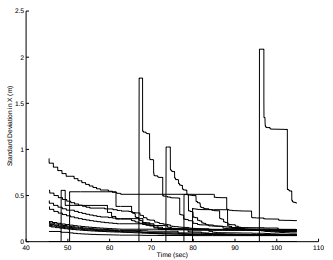
\includegraphics[width = 0.5\hsize]{figures/convergence_landmark_uncertainty.png}
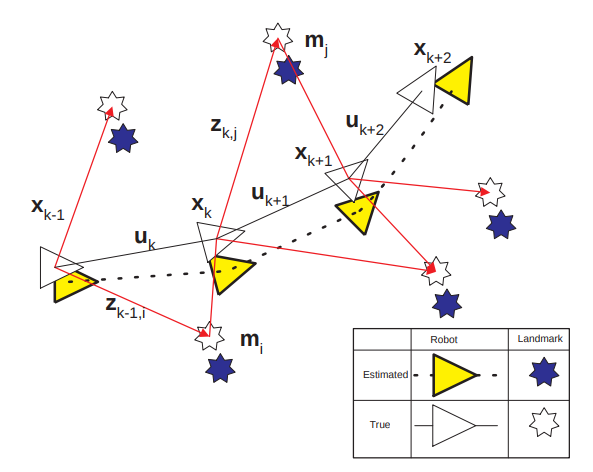
\includegraphics[width = 0.5\hsize]{figures/ess_slam.png}
\caption{Left: Graphical depiction of convergence in landmark uncertainty. Time history of standard deviations of a set of landmark locations. Over time, standard deviations reduce monotonically to a lower bound \cite{F_Durr_Pt1}. Right: Error between estimated and true landmarks is mostly common between landmarks.}
\label{slam_prob_fig}
\end{figure}






\newpage
\bibliographystyle{ieeetr}
\bibliography{bibliography.bib}
\end{document}

